\documentclass[../slides.tex]{subfiles}

\title{2018-2019 Inleiding Logica (KI1V13001) \\ Lecture 3}
 
\date{September 10, 2019\\[2ex] {\tiny \textcopyright~The non-copyrighted content of these slides is open access under \href{https://creativecommons.org/licenses/by-sa/4.0/}{CC BY-SA 4.0}}}
 
%%%%%%%%%%%%%%%

\begin{document}

\setcounter{framenumber}{63}
\begin{frame}
	\maketitle
\end{frame}

\begin{frame}{Overview}
\tableofcontents
\end{frame}

\section{Rehash}
\begin{frame}{Rehash}

\begin{itemize}

	\item You have to learn mathemateze like a foreign language.
	
	\item Variables stand for arbitrary but fixed objects, constants stand for known objects. 

	\item \alert{An object is defined by giving a list of properties that the object and only the object satisfies. We need to prove existence and uniqueness.}	
				
		\item \alert{A property or relation is defined by giving the conditions for an object has the property or some objects stand in the relation. It mustn't be circular.}
		
		\item  \alert{A mathematical proof is a rigorous, step-by-step argument which establishes the truth of a mathematical statement.} 

		\item Think of proving as problem solving. 
		
		\item Follow the advice!


\end{itemize}

\end{frame}

\section{3.0 Elementary Set Theory}
\subsection{3.1 Sets and Set Notation}

\begin{frame}{3.1 Sets and Set Notation}

	\begin{itemize}
	
		\item (3.1.1) A \emph{set} is a collection of objects, called its \emph{elements} or \emph{members}.
		
		\begin{itemize}
		
			\item $x\in X$ means $x$ is an element of $X$
			
			\item $x\notin X$ means $x$ is \emph{not} an element of $X$.
		
		\end{itemize}
		
		\item (3.1.2) \emph{Extensional Definition}. $\{a_1, \mathellipsis, a_n\}$ is the set whose members are $a_1, \mathellipsis, a_n$.
		
		\begin{itemize}
		
			\item  $\{1,a, \{\text{Robbie},0\}\}$ contains $1,a,0$ and the set (!) $ \{\text{Robbie}\}$
			
			\item $\{0\}$, singleton 0, contains only $0$			
			\item $\{ \}$ contains nothing, it's the \emph{empty set} and also denoted $\emptyset$
			
			\item $0$ is \emph{not} a set (note that $0\neq \{0\}$!)
		
		\end{itemize}

		\item (3.1.3) There are also \emph{infinite} sets:		
		
			\begin{itemize}
			
				\item $\mathbb{N}$ the set of natural numbers
				
				\item $\mathbb{Z}$ the set of integers
				
				\item $\mathbb{Q}$ the set of rationals
				
				\item $\mathbb{R}$ the set of reals
			
			\end{itemize} 
			
		\item Note that  $\{0,1,2,\mathellipsis\}$ is \emph{not} an extensional definition of $\mathbb{N}$! 
		
	\end{itemize}

\end{frame}

\begin{frame}{Set Abstraction}


	\begin{itemize}

		\item (3.1.6) If $X$ is the set of all objects satisfying condition $\Phi$, then $X$ can be written as the \emph{abstract} $\{x:\Phi(x)\}$:
		
		\begin{itemize}
		
			\item $\{x: x\in\mathbb{N}\text{ and }1\leq x\leq 10\}$ is the set of natural numbers between 1 and 10
			
			\item $\{x: x\text{ is prime}\}$ is the set of all prime numbers
		
		\end{itemize}
		
		\item An object $a$ is an element of $\{x:\Phi(x)\}$ iff $a$ satisfies the condition $\Phi$:
		
		\begin{itemize}
					
			\item $n\in \{x: x\in\mathbb{N}\text{ and }1\leq x\leq 10\}$ iff $n\in\mathbb{N}$ and $1\leq n\leq 10$
		
		\end{itemize}
		
		\item (3.1.7) Sometimes, we use set abstraction over an ambient set:
		
		\begin{itemize}
		
			\item $\{x\in \mathbb{N}:x\cdot x=2\}=\emptyset$
			
			\item $\{x\in \mathbb{R}:x\cdot x=2\}=\{\sqrt{2},-\sqrt{2}\}$
					
		\end{itemize}
		
		\item (3.1.8) Sometimes, we assume that the members of a set have a specific \emph{form}:
	
		\begin{itemize}
		
			\item $\{\frac{n}{m}:n,m\in \mathbb{Z},m\neq 0\}=\{x: \text{ there are }n,m\in \mathbb{Z}\text{ s.t. }x=\frac{n}{m},m\neq 0 \}$
		
		\end{itemize}
	
	\end{itemize}

\end{frame}

\begin{frame}{The Russel Paradox}

	\begin{itemize}
	
		\item Not every $\{x: \Phi(x)\}$ exists!
		
		\item For let $\Phi(x)$ be the condition $x\notin x$ and consider \[r:=\{x:x\notin x\}.\] 
		
		\item \emph{Russel's Paradox}. Assume that $r$ exists.  We know that $r\in r$ iff $r\notin r$.  But either (a) $r\in r$ or (b) $r\notin r$ (classical logic).  If (a) $r\in r$, then $r\notin r$.  Contradiction.  And if (b) $r\notin r$, then $r\in r$. Again, a contradiction.  So, either way, if we assume that $r$ exists (and classical logic), then we get a contradiction.  \hfill $\square$ 
		
		\item Solution: $r$ doesn't exist!
	
	\end{itemize}
	
	\begin{center}
		\begin{tabular}{c}
		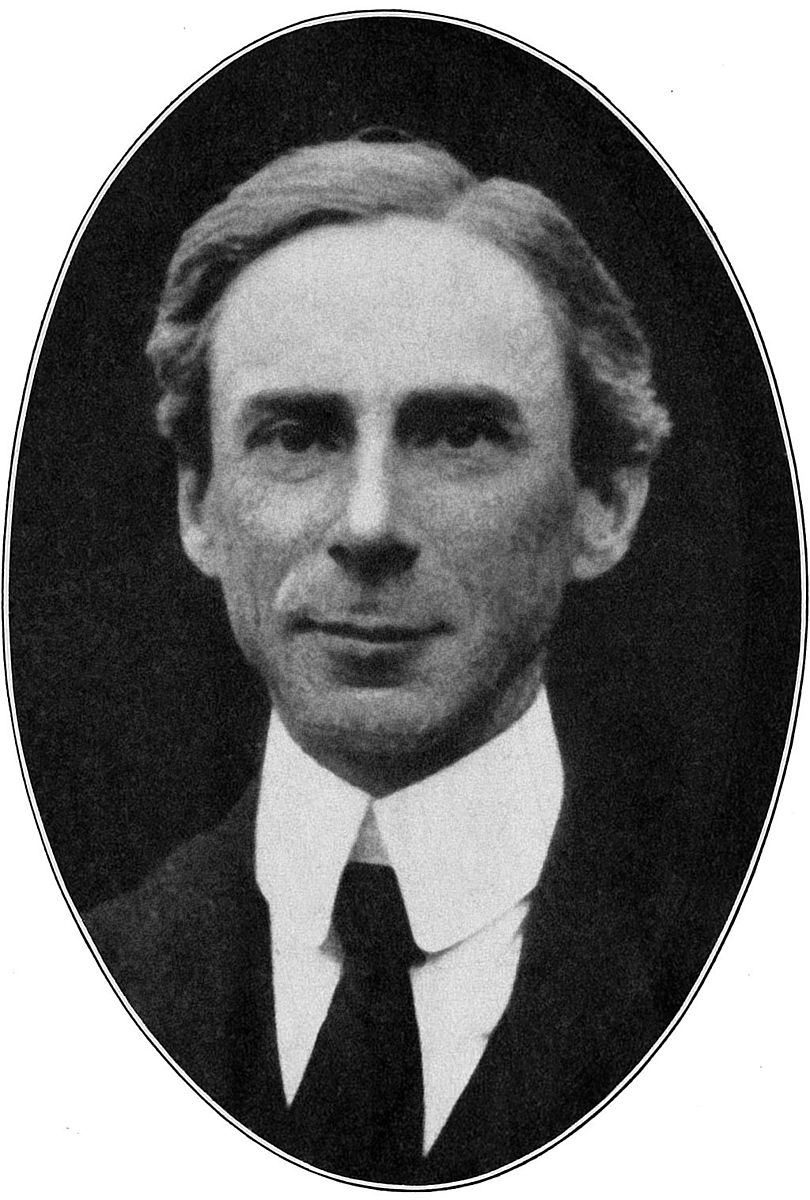
\includegraphics[width=10ex]{russel}\\[-1ex]
		{\tiny $\not\hspace{-1ex}\textcopyright$ Bertrand Russell (1916). Justice in War-Time. Chicago: The Open Court Publishing Co, work in public domain}
		\end{tabular}
		\end{center}
	

\end{frame}

\subsection{3.2 The Subset Relation}
\begin{frame}{3.2 The Subset Relation}
	
	\begin{itemize}
	
		\item (3.2.1) A set $X$ is a subset of a set $Y$ iff every member of $X$ is also a member of $Y$.
		
		\begin{itemize}
		
			\item $X\subseteq Y$ means $X$ is a subset of $Y$
			
			\item $X\nsubseteq Y$ means $X$ is \emph{not} a subset of $Y$
		
		\end{itemize}
		
		\item Note that $X\nsubseteq Y$ iff there exists an $x\in X$ such that $x\notin Y$!
		
		\item \emph{Examples}:
		
		\begin{itemize}
		
			\item $\{0,1\}\subseteq \{1,a,0,\{b,1\}\}$
			
			\item $\{b,1\}\nsubseteq \{1,a,0,\{b,1\}\}$ (but $\{b,1\}\in \{1,a,0,\{b,1\}\}$!)
			
			\item $\mathbb{N}\subseteq \mathbb{Z}$
			
			\item $\mathbb{Z}\nsubseteq \mathbb{N}$
		
		\end{itemize}
		
		\item Two facts:
		
			\begin{itemize}
			
				\item (3.2.2) For all $X$, $X\subseteq X$
				
				\item (3.2.4) For all $X$, $\emptyset\subseteq X$.
			
			\end{itemize}
	
	\end{itemize}

\end{frame}

\begin{frame}{Proof of 3.2.3}

	\begin{itemize}

		\item We show this fact indirectly. 
		
		\item So, suppose that there exists a set $X$ such that $\emptyset\nsubseteq X$. Call this set $A$. 
		
		\item We get that $\emptyset\nsubseteq A$, which means that there exists at least one object $x$ such that $x\in \emptyset$ but $x\notin A$. Call this object $a$. 
		
		\item We get that $a\in \emptyset$. 
		
		\item But we know that for each $x$, $x\notin \emptyset$, and hence $a\notin \emptyset$. 
		
		\item We've arrived at a contradiction, $a\in \emptyset$ and $a\notin\emptyset$. 
		
		\item Hence the assumption that there exists a set $X$ such that $\emptyset\nsubseteq X$ is false.
		
		\item So for each set $X$, we have that $\emptyset\subseteq X$.
		
		\item  $\qedsymbol$


\end{itemize}

\end{frame}

\begin{frame}{The Power Set}

	\begin{itemize}
	
		\item (3.2.5) For $X$ a set, we define the \emph{power set} $\wp(X)$ by \[\wp(X)=\{Y:Y\subseteq X\}\]
		
		\item \emph{Examples}.
		
			\begin{itemize}
			
				\item $\wp(\emptyset)=\{\alert{\emptyset}\}$
				
				\item $\wp(\{0\})=\{\alert{\emptyset}, \alert{\{0\}}\}$
			
				\item $\wp(\{a,b\})=\{\alert{\emptyset}, \{a\}, \{b\},\alert{\{a,b\}}\}$
				\item $\wp(\{a,b,c\})=\{\alert{\emptyset}, \{a\}, \{b\}, \{c\}, \{a,b\}, \{a,c\}, \{b,c\}, \alert{\{a,b,c\}}\}$
				
				\item \dots
			
			\end{itemize}
			
		\item Fact: If $X$ has $n$ members, then $\wp(X)$ has $2^n$ members. (This can be shown by mathematical induction, good exercise!)
		

	\end{itemize}

\end{frame}

\subsection{3.3 The Axiom of Extensionality}
\begin{frame}{3.3 The Axiom of Extensionality}

	\begin{itemize}
	
		\item (3.3.1) Sets are individuated by their members:
		
\begin{description}
	\item[Axiom of Extensionality.] For all sets $X$ and $Y$, $X=Y$ iff $X\subseteq Y$ and $Y\subseteq X$. 
\end{description}
		
	\item \emph{Examples}:
	
		\begin{itemize}
		
			\item $\{1,2\}=\{2,1\}$
			
			\item $\{b,a,a\}=\{a,b\}$
			
			\item $\{n\in\mathbb{Z}:z\text{ is even}\}=\{n\in\mathbb{Z}:\text{there is a }k\in \mathbb{Z}\text{, s.t. }n=2\cdot k\}$
		
		\end{itemize}
		
	\item (3.3.3) Let's say that a set $X$ is \emph{empty} iff for all objects $x$, we have that $x\notin X$. Then we have that for all sets $X$, if $X$ is empty, then $X=\emptyset$.

		
	\end{itemize}

\end{frame}

\begin{frame}{Proof of 3.3.3}

	\begin{itemize}

		\item We prove this indirectly. 
		
		\item So, suppose that there exists a set $X$ such that $X$ is empty but $X\neq\emptyset$.  Call this set $A$.
		
		\item It follows that $A\neq \emptyset$, hence either (a) $A\nsubseteq \emptyset$ or (b) $\emptyset\nsubseteq A$. 
		
		\item We've already established that $\emptyset\subseteq X$ for every set $X$, so (b) directly leads to a contradiction.
		
		\item We focus on case (a): $A\nsubseteq \emptyset$.
		
		\item If $A\nsubseteq \emptyset$, this means that there exists an object $x$ such that $x\in A$ but $x\notin \emptyset$. Call this object $a$. 
		
		\item We get that $a\in A$. But we've assumed that $A$ is an empty set, meaning that for all $x$, $x\notin A$. So, certainly, $a\notin A$. We've arrived at a contradiction, $a\in A$ and $a\notin A$.
		
		\item So, in both cases (a) and (b), we get a contradiction. 
		
		\item Hence, for all sets $X$, if $X$ is empty, then $X=\emptyset$.
		
		\item $\qedsymbol$
		
		\end{itemize}

\end{frame}

\subsection{3.4 Operations on Sets: Union, Intersection, Difference}
\begin{frame}{3.4 Operations on Sets: Union, Intersection, Difference}

	\begin{itemize}
	
		\item (3.4.1) The \emph{union} of two sets contains all the objects that are in at least one of the two sets:	
		\[X\cup Y=\{x: x\in X\text{ or }x\in Y\}.\]
		
		
		\item (3.4.2) The \emph{intersection} of two sets contains all things that are in both sets:
		 \[X\cap Y=\{x:x\in X\text{ and }x\in Y\}.\]
	
		\item (3.4.5) The \emph{difference} between one set and another are all the elements that are in the one but not the other: \[X\setminus Y=\{x\in X:x\notin Y\}.\]
		
		\item \emph{Examples}: Let $X=\{a,b\}$ and $Y=\{b,c\}$. Then:
		
		\begin{itemize}
		
			\item $X\cup Y=\{a,b,c\}$
			
			\item $X\cap Y=\{b\}$
			
			\item $X\setminus Y=\{a\}$
		
		\end{itemize}
	
	\end{itemize}

\end{frame}

\begin{frame}{Draw a Picture --- Venn Diagrams}

\begin{center}
	\begin{tabular}{c c}
		\begin{venndiagram2sets}[labelA=, labelB=, radius=1cm]%
    \fillACapB
    \setpostvennhook
    {
    \draw (labelA) ++(150:4ex) node{$X$};
%      \draw (labelA) ++(-105:8ex) node{$\scriptstyle\bullet$} ++(0,0) node[above]{$n_{i j} $};
    \draw (labelB) ++(20:5ex) node{$Y$};
    \draw (venn bottom right) ++(-2.125,0.3) node{$X\cap Y$};;
        }%
    \end{venndiagram2sets}
     &
 		\begin{venndiagram2sets}[labelA=, labelB=, radius=1cm]%
    \fillA \fillB
    \setpostvennhook
    {
    \draw (labelA) ++(150:4ex) node{$X$};
%      \draw (labelA) ++(-105:8ex) node{$\scriptstyle\bullet$} ++(0,0) node[above]{$n_{i j} $};
    \draw (labelB) ++(20:5ex) node{$Y$};
    \draw (venn bottom right) ++(-2.125,0.3) node{$X\cup Y$};;
        }%
    \end{venndiagram2sets}
    \\
     \begin{venndiagram2sets}[labelA=, labelB=, radius=1cm]%
    \fillOnlyA
    \setpostvennhook
    {
    \draw (labelA) ++(150:4ex) node{$X$};
%      \draw (labelA) ++(-105:8ex) node{$\scriptstyle\bullet$} ++(0,0) node[above]{$n_{i j} $};
    \draw (labelB) ++(20:5ex) node{$Y$};
    \draw (venn bottom right) ++(-2.125,0.3) node{$X\setminus Y$};;
        }%
    \end{venndiagram2sets}      
 	\end{tabular}

\textbf{A Venn Diagram is \emph{not} a proof!}

\end{center}

\end{frame}


\begin{frame}{A Proposition}

\begin{itemize}

	\item (3.4.3) For all sets $X$ and $Y$, if $X\cap Y=X$, then $X\subseteq Y$.
	
	\item \emph{Proof}.
		\begin{itemize}
		
			\item We use universal generalization and direct proof.
			
			\item So, let $A$ and $B$ be two sets and suppose that $A\cap B=A$.

			\item We need to show that for each $x$, if $x\in A$, then $x\in B$. 
			
			\item So take an arbitrary object $a$ and suppose that $a\in A$. 
			
			\item Suppose for indirect proof that $a\notin B$. 
			
			\item It's easily seen that $A\cap B=A$.
			
			\item Since $a\in A$ and $A=A\cap B$, it follows that $a\in A\cap B$. 
			
			\item But if $a\in A\cap B$, then also $a\in B$. 
			
			\item We have arrived at a contradiction, $a\in B$ and $a\notin B$. 
			
			\item Hence $a\in B$ by indirect proof.
			
			\item  So, if $a\in A$, then $a\in B$, i.e. $A\subseteq B$.
			
			\item  So, if $A\cap B=A$, then $A\subseteq B$.
			
			\item $\qedsymbol$

	\end{itemize}
	
	\end{itemize}

\end{frame}

\begin{frame}{A Picture}

\begin{center}
 \begin{venndiagram2sets}[labelA=X, labelB=Y, radius=2.5cm, overlap=2cm, labelAB={$X\cup Y=X$}]%
    \fillOnlyA
    \setpostvennhook
    {
%    \draw (labelA) ++(150:4ex) node{$X$};
%%      \draw (labelA) ++(-105:8ex) node{$\scriptstyle\bullet$} ++(0,0) node[above]{$n_{i j} $};
%    \draw (labelB) ++(20:5ex) node{$Y$};
%    \draw (venn bottom right) ++(-2.125,0.3) node{$X\setminus Y$};;
        }%
    \end{venndiagram2sets}  
    
    \textbf{A Venn Diagram is \emph{not} a proof!}

   \end{center}

\end{frame}

\subsection{3.5 Ordered-Pairs and Cartesian Products}
\begin{frame}{3.5 Ordered-Pairs and Cartesian Products}

	\begin{itemize}
	
		\item (3.5.1) An \emph{ordered pair} is a set-like collection of two objects, except that \emph{order matters}:
		
			\begin{itemize}
			
				\item $(a,b)$ is the ordered pair with $a$ in first and $b$ in second place
			
			\end{itemize}
			
		\item Note that $(2,1)\neq (1,2)$!
			
		\item (3.5.2) An \emph{(ordered) $n$-tuple} is a set-like collection of $n$-objects in that order:
		
		\begin{itemize}
		
			\item $(a_1, \mathellipsis, a_n)$ is the $n$-tuple with $a_i$ as the $i$-th component (for $1\leq i\leq n$).
		
		\end{itemize}
		
		\item Note that $(2,2,1)\neq (2,1)$!
		
		\item (3.5.4) The \emph{Cartesian product} of $X_1, \mathellipsis, X_n$ is the set of all $n$-tuples whose $i$-th component comes from $X_i$: \[X_1\times \mathellipsis\times X_n=\{(x_1, \mathellipsis, x_n):x_1\in X_1, \mathellipsis, x_n\in X_n\}.\]

		
		\item \emph{Examples}. 
		
		\begin{itemize}
		
			\item $\{1,2\}\times \{a,b\}=\{(1,a), (1,b), (2,a), (2,b)\}$
			
			\item $\{a,b\}\times \{1,2\}=\{(a,1), (a,2), (b,1), (b,2)\}$
			
			\item $\{1,2\}^2=\{1,2\}\times\{1,2\}=\{(1,1), (1,2), (2,1), (2,2)\}$
		
		\end{itemize}

	
	\end{itemize}

\end{frame}

\subsection{3.6 Properties, Relations. and Functions}
\begin{frame}{3.6 Properties, Relations. and Functions}

	\begin{itemize}
	
		\item (3.6.1) A \emph{property}, $P$, over a set of objects, $X$ is a set of elements of $X$, i.e. $P$ is a property over $X$ iff $P\subseteq X$.
	
		\item \emph{Example}. The property of being an even natural is $\{n\in\mathbb{N}:\text{there exists a }k\in\mathbb{N}\text{, such that }k\leq n\text{ and }n=2k\}$
		
		\item (3.6.3) An \emph{$n$-ary relation} over $X$, $R$, is simply a set of $n$-tuples of elements from $X$, i.e. $R\subseteq X^n$.
		
		\item \emph{Example}. The (binary) relation of smaller than over the reals is $\{(x,y)\in\mathbb{R}^2: x\leq y\}$.
	
	\end{itemize}

\end{frame}

\begin{frame}{Functions}

\vspace{-2ex}

	\[f(x)=2x^3-4x^2+2x-7\]

	\begin{itemize}
	
		\item A \emph{function}, $f$, from one set, $X$, to another, $Y$, assigns to each element $a\in X$ a \emph{unique} element $f(a)\in Y$:
		
		\begin{itemize}
		
			\item For all $a,b\in X$, if $f(a)\neq f(b)$, then $a\neq b$.
		
		\end{itemize}
		
		\item $f(0)=-7, f(1)=-7, f(2)=-3, \mathellipsis$
		
		\item Terminology:
			
			\begin{itemize}
			
				\item $X$ is the \emph{domain} of $f$, $X=dom(f)$
				
				\item $Y$ is the \emph{range} of $f$, $Y=rg(f)$
								
			\end{itemize}
			
		\item To define a function, we need to give a unique output for every input:
			
\begin{center}
	
\begin{tabular}{c c c}
  \begin{tikzpicture}[scale=.5,
     >=stealth,
     bullet/.style={
       fill=black,
       circle,
       minimum width=1pt,
       inner sep=1pt
     },
     projection/.style={
       ->,
       thick,
       shorten <=2pt,
       shorten >=2pt
     },
     every fit/.style={
       ellipse,
       draw,
       inner sep=0pt
     }
   ]
     \foreach \y/\l in {1/d,2/c/,3/b,4/a}
       \node[bullet,label=left:$\l$] (a\y) at (0,\y) {};
 
     \foreach \y/\l in {1/4,2/3,3/2,4/1}
       \node[bullet,label=right:$\l$] (b\y) at (4,\y) {};
 
     \node[draw,fit=(a1) (a2) (a3) (a4),minimum width=1.5cm] {} ;
     \node[draw,fit=(b1) (b2) (b3) (b4),minimum width=1.5cm] {} ;
 
     \draw[projection] (a4) -- (b4);
     \draw[projection] (a4) -- (b3);
     \draw[projection] (a2) -- (b3);
     \draw[projection] (a3) -- (b1);
     \draw[projection] (a4) -- (b3);
     \draw[projection] (a1) -- (b2);
   \end{tikzpicture}
   &
   \quad
   &
    \begin{tikzpicture}[scale=.5,
     >=stealth,
     bullet/.style={
       fill=black,
       circle,
       minimum width=1pt,
       inner sep=1pt
     },
     projection/.style={
       ->,
       thick,
       shorten <=2pt,
       shorten >=2pt
     },
     every fit/.style={
       ellipse,
       draw,
       inner sep=0pt
     }
   ]
     \foreach \y/\l in {1/d,2/c/,3/b,4/a}
       \node[bullet,label=left:$\l$] (a\y) at (0,\y) {};
 
     \foreach \y/\l in {1/4,2/3,3/2,4/1}
       \node[bullet,label=right:$\l$] (b\y) at (4,\y) {};
 
     \node[draw,fit=(a1) (a2) (a3) (a4),minimum width=1.5cm] {} ;
     \node[draw,fit=(b1) (b2) (b3) (b4),minimum width=1.5cm] {} ;
 
     \draw[projection] (a4) -- (b4);
     \draw[projection] (a2) -- (b1);
     \draw[projection] (a3) -- (b1);
   \end{tikzpicture}
   
   \\
   
   More than one value for $a$ & & No value for $d$
   
   \end{tabular}
  \end{center}
 
	
	\end{itemize}

\end{frame}

\begin{frame}{A Function?}

	\begin{center}
	\begin{tikzpicture}[scale=1,
     >=stealth,
     bullet/.style={
       fill=black,
       circle,
       minimum width=1pt,
       inner sep=1pt
     },
     projection/.style={
       ->,
       thick,
       shorten <=2pt,
       shorten >=2pt
     },
     every fit/.style={
       ellipse,
       draw,
       inner sep=0pt
     }
   ]
     \foreach \y/\l in {1/1,2/2/,3/3,4/4}
       \node[bullet,label=left:$\l$] (a\y) at (0,\y) {};
 
     \foreach \y/\l in {1/4,2/3,3/2,4/1}
       \node[bullet,label=right:$\l$] (b\y) at (4,\y) {};
 
     \node[draw,fit=(a1) (a2) (a3) (a4),minimum width=1.5cm] {} ;
     \node[draw,fit=(b1) (b2) (b3) (b4),minimum width=1.5cm] {} ;
 
     \draw[projection] (a4) -- (b1);
     \draw[projection] (a3) -- (b2);
     \draw[projection] (a2) -- (b3);
     \draw[projection] (a1) -- (b4);
   \end{tikzpicture}
   
      \onslide<2>{$f:\{1,2,3,4\}\to\{1,2,3,4\}$, $f(x)=x$}

   \end{center}
   

\end{frame}

\begin{frame}{Binary Functions}

	\begin{itemize}
	
		\item A special case, we'll often encounter are functions where $dom(f)=X^2$ for some set $X$.
		
		\item \emph{Example} $f:\{a,b,c\}^2\to \{0,1\}$ defined by:
		
		\begin{center}
	\begin{tabular}{c c c c c c c c c c c}
	$(a,a)$ & $\overset{f}{\mapsto}$ & 0 & \quad & (b,a) & $\overset{f}{\mapsto}$ & 0  \quad & (c,a) & $\overset{f}{\mapsto}$ & 1\\

	$(a,b)$ & $\overset{f}{\mapsto}$ & 1 & \quad & (b,b) & $\overset{f}{\mapsto}$ & 0  \quad & (c,b) & $\overset{f}{\mapsto}$ & 1\\


	$(a,c)$ & $\overset{f}{\mapsto}$ & 1 & \quad & (b,c) & $\overset{f}{\mapsto}$ & 1  \quad & (c,c) & $\overset{f}{\mapsto}$ & 0\\


	\end{tabular}
\end{center}

	\item This assignment can be given in table form:

\begin{center}
	\begin{tabular}{ c | c c c}
	$f$ & $a$ & $b$ & $c$ \\ \hline
	
	$a$ & 0 & 1 & 1\\
	
	$b$ & 0 & 0 & 1\\
	
	$c$ & 1 & 1 & 0
	
	\end{tabular} 
	
\end{center}
	
	\end{itemize}

\end{frame}

\subsection{3.7 Inductive Definitions and Proof by Induction}
\begin{frame}{3.7 Inductive Definitions and Proof by Induction}

	\begin{itemize}
	
		\item How can we ``properly'' define $\mathbb{N}$?
		
		\item (3.7.1) We want to say that $\mathbb{N}$ is ``the set of 0 and all its successors.''
		
		\item Idea:
		
		\begin{itemize}
		
			\item $0\in\mathbb{N}$
			
			\item For all $n$, if $n\in\mathbb{N}$, then $n+1\in\mathbb{N}$
			
			\item ``Nothing else is in $\mathbb{N}$.
		
		\end{itemize}
	
		\item In this way we can easily show that $3\in\mathbb{N}$, since:
		
		\begin{itemize}
		
			\item $0\in\mathbb{N}$
			
			\item $1=0+1$, so $1\in\mathbb{N}$
			\item $2=1+1$, so $2\in\mathbb{N}$
			\item $3=2+1$, so $3\in\mathbb{N}$
			
		\end{itemize}
		
		\item To show that $\frac{1}{2}\notin \mathbb{N}$, we'd need to show that there exists no $n\in\mathbb{N}$ such that $n+1=\frac{1}{2}$.
		
		\item (3.7.3) That's tricky! $\frac{1}{2}\notin \mathbb{N}\Rightarrow -\frac{1}{2}\notin\mathbb{N}\Rightarrow -\frac{3}{2}\notin\mathbb{N}\Rightarrow\mathellipsis.$
	
	\end{itemize}

\end{frame}

\begin{frame}{A Proper Definition of $\mathbb{N}$}

	\begin{itemize}

		\item What does it mean that ``nothing else is a member of $\mathbb{N}$''?
		
		\item (3.7.7) We say that one set $X$ is \emph{smaller than} a set $Y$ iff $X\subseteq Y$.
		
		\item $\mathbb{N}$ is the smallest set such that:
		
		\begin{enumerate}[(i)]
	
		\item $0\in X$
		
		\item For all numbers $x$, if $x\in X$, then $x+1\in X$.
	
	\end{enumerate}
	
		\item (3.7.8) With this official definition, we can prove that $\frac{1}{2}\notin \mathbb{N}$.
		
		\item \emph{Proof} (Sketch). Suppose that $X$ satisfies (i) and (ii) and $\frac{1}{2}\in X$. Then $Y=X\setminus \{\frac{k}{2}: k\in \mathbb{Z}\text{ and }k\text{ is odd}\}$ also satisfies (i) and (ii) and is smaller than $X$. So $X$ cannot be $\mathbb{N}$. Hence if $\frac{1}{2}\in\mathbb{N}$, then $\mathbb{N}\neq\mathbb{N}$. Contradiction. So $\frac{1}{2}\notin\mathbb{N}$. $\qedsymbol$
	
	\end{itemize}

\end{frame}

\begin{frame}{Function Recursion (3.7.3)}

	\begin{itemize}
	
		\item We can use function recursion on $\mathbb{N}$:
		
		\item \emph{Example}. We define $f:\mathbb{N}^2\to\mathbb{N}$ as follows
	\begin{enumerate}[(i)]
	
		\item For every number $n\in\mathbb{N}$, $f(n, 0)=0$.
		
		\item For all numbers $n,m\in\mathbb{N}$, $f(n,m+1)=f(n,m)+n$.
	
	\end{enumerate}
	
	\item Since the numbers are $0$ and all its successors, this gives us a value for each $n$.
	
	\item \emph{Example}: $f(3,2)=\dots$
	
	\begin{itemize}
		
		\item $f(3,1+1)=f(3, 1)+3$
		
		\item $f(3,1)=f(3,0+1)=f(3,0)+3$ and $f(3, 0)=0$
			
		\item $f(3,1)+3=f(3,0+1)+3=(f(3, 0)+3)+3=(0+3)+3=6$.
	
	\end{itemize}

		
	\end{itemize}
	
	\begin{center}
		\begin{tabular}{c}
		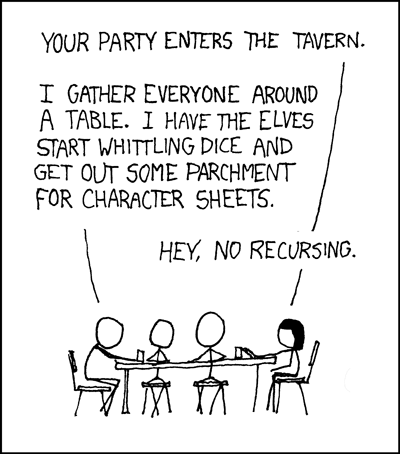
\includegraphics[width=15ex]{xkcd-recursion}\\[-1ex]
		{\tiny \textcopyright~\url{https://xkcd.com/244/}, CC BY-NC 2.5}
		\end{tabular}
		\end{center}

\end{frame}

\begin{frame}{Proof by Induction (3.7.4)}

	\begin{itemize}
	
	
		\item For every inductively defined set, we can prove things about its members via \emph{proof by induction}:
		
		\begin{itemize}
		
			\item (3.7.9) \textbf{Theorem}. Suppose that $\Phi$ is a condition on numbers such that:
		\begin{enumerate}[(i)]
		
			\item $\Phi(0)$ (`base case')
			
			\item for all natural numbers $n\in\mathbb{N}$, if $\Phi(n)$, then $\Phi(n+1)$. (`induction step')
		
		\end{enumerate}
		
		\item \emph{Proof}. Let $\Phi$ be an arbitrary condition on numbers satisfying conditions (i) and (ii), Consider the set $\{x:\Phi(x)\}$. By the conditions (i) and (ii) of our theorem, $\{x:\Phi(x)\}$ satisfies conditions (i) and (ii) from the definition of $\mathbb{N}$. Since $\mathbb{N}$ is the smallest set satisfying those conditions, we have that $\mathbb{N}\subseteq\{x:\Phi(x)\}$. But now, it easily follows that for all $n\in\mathbb{N}$, we have that $\Phi(n)$. For let $n\in\mathbb{N}$ be an arbitrary number. Since $\mathbb{N}\subseteq\{x:\Phi(x)\}$, it follows that $n\in\{x:\Phi(x)\}$. But that just means that $\Phi(n)$, as desired.
		
		\end{itemize}
		
		\item It's a kind of ``domino principle.''
	
	\end{itemize}


\end{frame}

\begin{frame}{Proof by Induction --- Example (3.7.5)}

Let $f:\mathbb{N}^2\to\mathbb{N}$ be defined by  follows
	\begin{enumerate}[(i)]
	
		\item For every number $n\in\mathbb{N}$, $f(n, 0)=0$.
		
		\item For all numbers $n,m\in\mathbb{N}$, $f(n,m+1)=f(n,m)+n$.
	
	\end{enumerate}
Then for all $n,m\in\mathbb{N}$, $f(n,m)=n\cdot m$.

\emph{Proof}:

\begin{itemize}

	\item \emph{Base case}: By (i), $f(n,0)=0$. Since $n\cdot 0=0$ for all $n\in\mathbb{N}$, the claim holds.
	
	\item \emph{Induction Step}: Let $n,m\in\mathbb{N}$ be arbitrary numbers and assume that $f(n,m)=n\cdot m$ (`induction hypothesis'). We know that $f(n,m+1)=f(n,m)+n$. By the induction hypothesis, we get {\small\[f(n,m+1)=f(n,m)+n=(n\cdot m)+n=n\cdot (m+1),\]} which is what we needed to show.
	
\end{itemize}
\end{frame}

\begin{frame}{Inductive Definitions Generalized}

	\begin{itemize}
	
		\item (3.7.10) In order to inductively define a set:
		
		\begin{enumerate}[1.]
	
		\item We give a set of initial elements.
		
		\item We provide a list of \emph{constructions} that allow us to form new elements from old elements.
		
		\item We define our set as the smallest set that contains all the initial elements and that is \emph{closed under} the constructions.
	
	\end{enumerate} 
	
		\item \emph{Example}. $Gargle$ is now defined as the smallest set $X$ such that:
			
			\begin{enumerate}[(i)]
			
				\item $\{\clubsuit,\spadesuit\}\subseteq X$.
			
				\item \begin{enumerate}[(a)]
				
					\item For all $x$, if $x\in X$, then $\diamondsuit x\diamondsuit\in X$.
			
					\item For all $x$, if $x,y\in X$, then $ x\heartsuit y\in X$.
				
				\end{enumerate}
				
			\end{enumerate}
			
		\item We get:
		
		\begin{itemize}
				
					\item $\clubsuit,\spadesuit\in Gargle$
					
					\item $\diamondsuit\clubsuit\diamondsuit,\diamondsuit\spadesuit\diamondsuit\in Gargle$
					
					\item $\clubsuit\heartsuit\clubsuit, \clubsuit\heartsuit\spadesuit, \spadesuit\heartsuit\spadesuit\in Gargle$
				
					\item $\clubsuit\heartsuit\diamondsuit\clubsuit\diamondsuit, \diamondsuit\spadesuit\diamondsuit\heartsuit\spadesuit,\mathellipsis\in Gargle$

				
				\end{itemize}
	
	\end{itemize}

\end{frame}

\begin{frame}{Function Recursion Generalized}

	\begin{itemize}
	
		\item (3.7.12) To recursively define a function on an inductively defined set:
		\begin{enumerate}[1.]
		
			\item We say what the value of our function is on the initial elements.
			
			\item We say how to calculate the value of the function for an element built by a construction, where we can reference to the values of the function for the elements the element is constructed from.
		
		\end{enumerate}
		
	\item (3.7.13) \emph{Example}: The function $\#_\spadesuit:Gargle\to\mathbb{N}$ is defined by the following recursion:
		
	\begin{enumerate}[(i)]
		
			\item $\#_\spadesuit(x)=\begin{cases} 1 & \text{if }x=\spadesuit
			\\0 &\text{if }x=\clubsuit\end{cases}$
			
			\item \begin{enumerate}[(a)]
					
					\item  $\#_\spadesuit( \diamondsuit x\diamondsuit)=\#_\spadesuit(x)$

					\item $\#_\spadesuit(x\heartsuit y)=\#_\spadesuit(x)+\#_\spadesuit(y)$		
		\end{enumerate}
		
	\end{enumerate}
	
	\item We get, for example:{\small\[\#_\spadesuit(\spadesuit\heartsuit\diamondsuit\spadesuit\diamondsuit)=\#_\spadesuit(\spadesuit)+\#_\spadesuit(\diamondsuit\spadesuit\diamondsuit)=\#_\spadesuit(\spadesuit)+\#_\spadesuit(\spadesuit)=1+1=2.\]}
	
	\end{itemize}

\end{frame}

\begin{frame}{An Issue with Gargles}

	\begin{itemize}
	
		\item The gargle $\spadesuit\heartsuit\clubsuit\heartsuit\spadesuit$ can constructed in two ways: 
		\begin{itemize}
		
			\item Since $\spadesuit,\clubsuit\in Gargle$, we know that $\clubsuit\heartsuit\spadesuit\in Gargle$. Since $\spadesuit\in Gargle$ and $\clubsuit\heartsuit\spadesuit\in Gargle$, we have $\spadesuit\heartsuit\clubsuit\heartsuit\spadesuit\in Gargle$
		
			\item Since $\clubsuit,\spadesuit\in Gargle$, we know that $\spadesuit\heartsuit\clubsuit\in Gargle$. Since $\spadesuit\in Gargle$ and $\spadesuit\heartsuit\clubsuit\in Gargle$, we have $\spadesuit\heartsuit\clubsuit\heartsuit\spadesuit\in Gargle$
		
		\end{itemize}
		
		\item This means that function recursion on gargles doesn't automatically work:
		
		\begin{enumerate}[(i)]
		
			\item $f(\spadesuit)=1$ and $f(\clubsuit)=0$
			
			\item \begin{enumerate}[(a)]
			
				\item $f(\diamondsuit x\diamondsuit)=f(x)$
				
				\item $f(x\heartsuit y)=\begin{cases}
			1 & \text{if }f(x)=1\text{ and }f(y)=0\\
			0 &\text{ otherwise}
			\end{cases}$
			
			\end{enumerate}
			
		\end{enumerate}	
					
		\item We get: 
		
		\begin{itemize}
		
			\item $f(\spadesuit\heartsuit\clubsuit\heartsuit\spadesuit)=1$ 
			
			\item $f(\spadesuit\heartsuit\clubsuit\heartsuit\spadesuit)=0$
		
		\end{itemize}
		
		\item \frownie
		
		\item We want \emph{unique readability}!
		
	\end{itemize}


\end{frame}

\begin{frame}{Inductive Proofs Generalized}

	\begin{itemize}
	
		\item To prove that all elements of an inductively defined set have satisfy a condition, we show:
		
		\begin{enumerate}[1.]
			
			\item All the initial elements satisfy the condition. (`base case')
			
			\item A newly constructed element satisfies the condition, whenever the elements that it's constructed from does. (`induction steps')
		
		\end{enumerate}
		
		\item \emph{Example}: Suppose that $\Phi$ is a condition on gargles. If we can show:
			\begin{enumerate}
			
				\item $\Phi(\clubsuit),$ and $\Phi(\spadesuit)$
				
				\item \begin{enumerate}\item For all gargles $x\in Gargle$, if $\Phi(x)$, then $\Phi(\diamondsuit x\diamondsuit)$.
			
					\item  For all gargles $x,y\in Gargle$, if $\Phi(x)$ and $\Phi(y)$, then $\Phi(x\heartsuit y)$
					
					\end{enumerate}
			\end{enumerate}
			Then for all gargles $x\in Gargle,$ $\Phi(x)$.
	
	\end{itemize}

\end{frame}

\begin{frame}{Example}

	\begin{itemize}

		\item \textbf{Proposition}. Each gargle contains at least one of $\spadesuit,\clubsuit$.
		
		\item \emph{Proof}.
		
			\begin{itemize}

				\item We prove this by induction over gargles.
				
				\item \emph{Base case}. There are two initial elements, $\spadesuit,\clubsuit$, each of which contains at least one of $\spadesuit,\clubsuit$.
				
				\item \emph{Induction Steps}. \begin{itemize}
				
					\item Suppose that $x$ contains at least one of $\spadesuit,\clubsuit$ (`induction hypothesis'). Consider $\diamondsuit x \diamondsuit$. Since by the induction hypothesis, $x$ contains one of $\spadesuit,\clubsuit$, and $\diamondsuit x \diamondsuit$ contains $x$, also $\diamondsuit x \diamondsuit$ contains at least one of $\spadesuit,\clubsuit$.
					
					\item Suppose that  both $x$ and $y$ contain at least one of $\spadesuit,\clubsuit$ (`induction hypothesis'). Consider $ x \heartsuit y$. Since by the induction hypothesis, $x$ contains one of $\spadesuit,\clubsuit$, and $x \heartsuit y$ contains $x$, also $x \heartsuit y$ contains at least one of $\spadesuit,\clubsuit$.

				
				\end{itemize}
				
				\item By the principle of induction over the gargles, we can conclude that all gargles contain at least one of $\spadesuit,\clubsuit$.

			\end{itemize}
	
	\end{itemize}

\end{frame}


\begin{frame}{How to Write (Generalized) Inductive Proofs}


	\begin{enumerate}[1.]
		
			\item State clearly that you're using induction to prove the claim.
			
			\item Prove the base case. 
			
			\item State clearly that you're now considering the induction steps. In each sub-case, begin by stating your induction hypothesis and then use it to derive the claim about the constructed element.
			
			\item State clearly that you're using induction to infer that the claim in question holds for all elements of the set.
		
		\end{enumerate}
		

\end{frame}

\begin{frame}{Core Ideas (Lecture Version)}
	
\begin{itemize}

		\item A set is a collection of objects, its elements.
		
		\item One set is a subset of another just in case all the elements of the one set are elements of the other. 
				
		\item Two sets are identical iff they have precisely the same elements. 
		
		\item The union of two sets contains any element of either set, their intersection contains only the objects that are in both sets. The difference of one set and another contains all the elements of the one but not the other.
		
		\item An ordered tuple is a a set-like collection of objects with a specific order. In tuples, order and multiplicity count.
		
		\item The Cartesian product of two sets contains all the tuples formed from those sets.
		
		\end{itemize}
		
	\end{frame}
		
\begin{frame}{Core Ideas (Lecture Version, Cont'd)}
	
\begin{itemize}
			
		\item A property is a set of objects. An $n$-ary relation is a set of $n$-tuples.
		
		\item A function assigns to each input a \emph{unique} output.
		
		\item To inductively define a set, we give a set of initial elements and a set of constructions for new elements.
		
		\item To recursively define a function, we give the value of the function for the initial elements and say how to calculate the value of a newly constructed element based on the values of the elements its constructed from.
		
		\item To prove a claim by induction over an inductively defined set, we show that all initial element satisfy the claim and that every newly constructed element satisfies the claim whenever the elements that it's constructed from do.
			

	\end{itemize}


\end{frame}

\begin{frame}

	\begin{center}
	{\huge\bf Thanks!}
	\end{center}

\end{frame}

\end{document}
